\documentclass{article}
\usepackage{hyperref}
\usepackage[margin = 1in]{geometry}
\usepackage{listings}
\usepackage{mathtools}
\usepackage{apacite}
\usepackage{graphicx} \graphicspath{ {./Images/} }
\usepackage{blindtext}
\usepackage{titling}
\usepackage{setspace} \doublespacing
\usepackage{wrapfig} 
\setlength\parindent{24pt}
\renewcommand\maketitlehooka{\null\mbox{}\vfill}
\renewcommand\maketitlehookd{\vfill\null}



\title{Spiking Neural Networks}
\author{Arslan Salikhov \\
	\and 
	Erik Caceros \\
	\and
	Brandon Lam \\
	}
\date{\today}



\begin{document}

\begin{titlingpage}
\maketitle
\begin{abstract}
	Use of Deep Neural Network, commonly referred to as
	\emph{deep learning} spiked in recent years and has been used
	as a tool for impressive advancements in the field of 
	\emph{Artificial Intelligence (AI)}
	Spiking Neural Networks draw inspiration from the 
	Purpose of this project is to demonstrate the capabilities of a 
	Spiking Neural Network and compare it to a more conventional 
	Object Recognition Deep Neural Network
	\end{abstract}
\end{titlingpage}


\tableofcontents
\newpage




\section{Architecture of the Spiking Neural Network}

When it comes to building a neural network, one has to establish an
architecture or an arrangement of layers and how they connect with each other.
It is particularly important, when the network increases in complexity. Object
classification + localization being a demanding task for a network to solve,
we have adopted a published and well-tested architecture for the task --
ResNet.

\subsection{ResNet}


\begin{wrapfigure}{r}{0.6\textwidth}
	\begin{center}
		\scalebox{0.5}{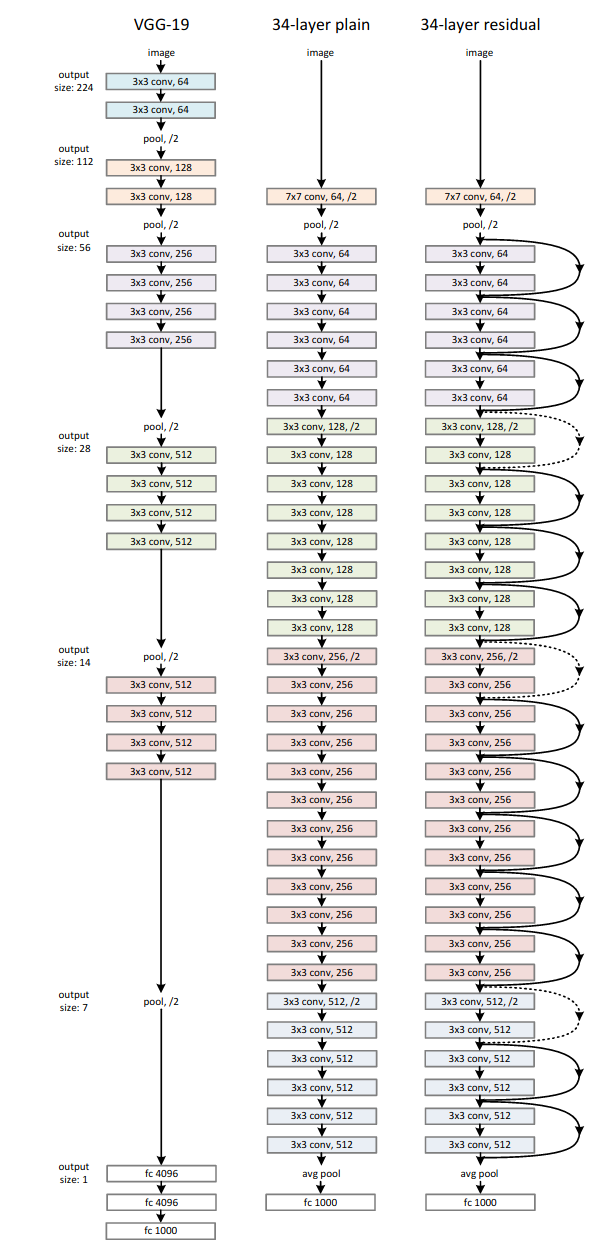
\includegraphics{resnet_comp.png}}
	\end{center}
	\caption{Architectures of VGG/Plain Network/ResNet}
\end{wrapfigure}

ResNet is named for its property, where convolutional layers of the network
are residually connected with each other using shortcut connections
(\citeA{resnet}). According to the authors of the original paper on ResNets,
addition of residual connections improves model's convergence, or ability for
model's loss to move towards a minimum with a decreasing trend. Meanwhile,
ResNets converge faster than their plain counterparts, the complexity of 
ResNets is much lower than complexity of well established Visual Geometry
Group (VGG) Networks given the same depth (3.6 billion FLOPs (Float Point 
Operations) vs. 19.6 billion FLOPs) (\citeA{resnet}).


\newpage
\bibliographystyle{apacite}
\bibliography{report}

\end{document}